\documentclass[12pt]{article}
\usepackage{geometry}
\usepackage{booktabs}
%-----------------------------format.tex-----------------
\usepackage{amsmath,amssymb}
\usepackage{graphicx}
\usepackage{fancybox}
\usepackage{fancyhdr}
\usepackage{lastpage}
\usepackage{hyperref}
\hypersetup{
    unicode={true},pdfstartview={FitH},pdfborder={0 0 0},
    colorlinks,linkcolor=blue,citecolor=blue,hyperindex,plainpages=false,}
% style: page layout
\setlength{\headheight}{15pt}
\setlength{\headsep}{20pt}
\setlength{\footskip}{30pt}
\setlength{\voffset}{-5pt}
\setlength{\hoffset}{16pt}
\setlength{\oddsidemargin}{0pt}
\setlength{\evensidemargin}{\oddsidemargin}
\setlength{\marginparpush}{0pt}
\setlength{\marginparwidth}{0pt}
\addtolength{\textheight}{3\baselineskip}
\hypersetup{
	colorlinks=true,
	linkcolor=black
}
\newtheorem{definition}{{definition}}
\newcounter{numdefinition}
\renewenvironment{definition}[1]
{\noindent\stepcounter{numdefinition}
\slshape Definition \arabic{numdefinition} \textsf{#1 :}
\begin{quote}\small\itshape}
{\end{quote}}

\newcommand{\dd}{\ensuremath{\,\mathrm{d}}}
%===============================================================
\fancypagestyle{plain}%���¶���plain��ʽ,����summary sheet
{\fancyhf{}
\setlength{\headheight}{0pt}\setlength{\headsep}{0pt}
\setlength{\voffset}{-50pt}\setlength{\oddsidemargin}{0pt}}

\graphicspath{{pic/}}
%=========================����ҳü===============================
\pagestyle{fancy} 
\rhead{page\thepage\ of \pageref{LastPage}}
\chead{} \lhead{Team \footnotesize{\#} 201906177} \lfoot{}
\cfoot{\thepage}
\rfoot{}
\renewcommand{\headrulewidth}{0.4pt}

\begin{document}

%=========================summary sheet.tex========================

\thispagestyle{empty}
\begin{minipage}{0.3\textwidth}
%\begin{flushleft}
%For office use only\\
%   T1\ \rule{3cm}{0.5pt}\\
%   T2\ \rule{3cm}{0.5pt}\\
%   T3\ \rule{3cm}{0.5pt}\\
%   T4\ \rule{3cm}{0.5pt}\\
%\end{flushleft}
\end{minipage}\hspace{\fill}
\begin{minipage}{0.3\textwidth}
\centering
Team Control Number\\[5pt]
\fontsize{20pt}{\baselineskip}\selectfont  \textbf{201906177} \normalsize\\[10pt]
Problem Chosen\\[5pt]
\fontsize{18pt}{\baselineskip}\selectfont \textbf{A }\normalsize\\
\end{minipage}\hfill
\begin{minipage}{0.35\textwidth}
%\begin{flushright}
%\shortstack[l]{
%For office use only\\
%   F1\ \rule{3cm}{0.5pt}\\
%   F2\ \rule{3cm}{0.5pt}\\
%   F3\ \rule{3cm}{0.5pt}\\
%   F4\ \rule{3cm}{0.5pt}}
%\end{flushright}
\end{minipage}\vspace*{10pt}
\rule{\textwidth}{0.5pt}

\begin{center}
  \textbf{ShuWei Cup}
\end{center}
%\enlargethispage
\noindent
{\Large \textbf{Summary}}
\vspace{7pt}

%==========================abstract.tex================================
aaaaaaaaaaaaaaaaaaaaaaaaaaaaaaa

\textbf{keyword}: sweet spot; corked bat; coefficient of restitution;%xxx speed; finite element method; 
\newpage

%====================Ŀ¼ҳ========================================
\thispagestyle{empty}
\setcounter{page}{0}
{\begin{center}\Large \textbf{}\end{center}}
\tableofcontents                                                  %
\newpage                                                          %
%==================================================================

\newcommand{\vw}{\frac{v_i}{\omega_i}}

%=======================\input{introduction1}=======================

\section{Introduction}	
\subsection{Background}

\subsection{Work}

%============================\input{definitions1}===========
\section{Problem Analysis}
\paragraph{Analysis of task one}

Make reasonable predictions of the aging trend of China and the medical needs of the residents according to the data of residents' income, age structure of the population and the economic development level etc. in the relevant statistical analysis data of the National Bureau of Statistic. 
According to the relevant data from 2009 to 2018 in the National Bureau of statistics, the group first selects appropriate indicators and then establishes a grey prediction model to predict and analyze the population aging trend and residents' medical needs of the epidemic in 2009-2018. Then, through the Markov model, the data from 2009-2018 simulates the distribution of residual in each interval and calculates the expectation of the predicted residual in 2019-2021 Value. Finally, the prediction results and residual expectation are made to be different, and the inherent deviation of traditional grey prediction is corrected. Through the combination of the two models, the goal of scientific prediction of the future development of population aging and the trend of residents' medical needs is achieved. Its thought flow chart is shown in Figure ~\ref{lct}~ :


\paragraph{Analysis of task two}

\paragraph{Analysis of task three} 
The question three ask us to propose a common queuing theory method and figure its related optimal queuing for this kind of queuing problem.Via refering to the operational mode of the real world hospital, we choose to adopt the $M/M/c/\infty$ model as the required theory. Then we acquire the hospital statistics and abstract the data into the parameter in model. Finally, to get the social cost to be lowest, we manage to find the optimized systems design for the queuing model.

\paragraph{Analysis of task four}

\paragraph{Analysis of task five}
%=======================\input{Assumptions1}=====================================
	\section{Symbol and Assumptions}
\subsection{Symbol Description}
\begin{center}
\begin{tabular}{ll}
	\hline
	symbols&definitions\\
	\hline
	$v_i$& velocity of ball before collision\\
	$v_f$& velocity of ball after collision\\
	$V_f$& velocity of bat after collision\\
	$S$ & the shear modulus the bat\\
	$Y$ & Young��s modulus of the bat\\
	\hline
\end{tabular}
\end{center}


\subsection{Fundamental assumptions}
\begin{enumerate}
%\item The bat is rigid, so there is no vibration in the bat(for the basic model).
%\item The ball hit and rebound perpendicular to the bat and is in the plane of the swing.
%\item The ball can be considered as a linear spring with friction.
%\item The bat is a free object in collision,and both ends of the bat is completely free.
%\item The vibration of the bat is harmonic(for augmented model).
\item The hourly wage of patient could be considered as the cost dissipated in queuing. And the hourly wage of  doctor could be seen as the cost of cost of service.
\end{enumerate}

%=============================\input{ModelforCollision}==========================
\section{Establishment and solution of the model}

 \subsection{The model of Problem 1}
	\subsubsection{Establishment of model}   
	\paragraph{GM(1,1)}The total number of cases in 2009-2018 is time series:
	
	 \begin{gather*}
	X^{(0)}=[x^{(0)}(1),x^{(0)}(2),\cdots,x^{(0)}(10)]
	\end{gather*}
	
	
	Generate a 1-AGO sequence by one accumulation:
	\begin{gather*}
	X^{(1)}=[x^{(1)}(1),x^{(1)}(2),\cdots,x^{(1)}(10)]
	\end{gather*}
	
	In the formula:$x^{(1)}(k)=\sum_{i=1}^{k}x^{(1)}(i),k=1,2,\cdots,10$.

Establish a differential equation based on the 1-AGO sequence as:\begin{gather}\label{333}
\frac{d X^{(1)}}{dt}+a X^{(1)} = u
\end{gather}

In the formula:$a$ is Develop grayscale,$u$ is Endogenous control grayscale.Let $\widehat{\alpha}$ be the parameter vector to be estimated and $\widehat{\alpha }=[a,u]^T$, be found by least squares method:
\begin{gather}
\widehat{\alpha }=(B^TB)^{-1}B^{T}Y_{n}
\end{gather}


Solving equation~\ref{333}~,The preliminary prediction model for the $k+1$ aging is available:

\begin{gather}
\widehat{X}(k+1)=[X^{(0)}(1)-\frac{u}{a}]e^{-ak}+\frac{u}{a},k=1,2,\cdots,16
\end{gather}

Similarly, the death number is taken as the vector $X^{(0)}=[x^{(0)}(1),x^{(0)}(2),\cdots,x^{(0)}(10)]$ Bring in the model to obtain the 2019-2021 death number grayscale prediction value.
	     
	     \paragraph{Markov model correction}
The Markov model is used to estimate the state and state probability of the GM(1,1) prediction error term, and the predicted value of the predicted state is used to correct the GM(1,1) prediction value. The state is divided by the 2009-2018 forecast data and the real data residual, and the residual sequence is:
\begin{gather*}
\varepsilon =[\varepsilon(1) ,\varepsilon(2), \cdots,\varepsilon(10)]
\end{gather*}

Absolute maximum residual value $\delta _{max}=\underset{1\leqslant i\leqslant13 }{max}\left | \varepsilon(i) \right |$.The prediction error is divided into three states. Let $\lambda =\frac{\delta _{max}}{6}$. The status is$E_{1}:(-3\lambda,-\lambda)$,$E_{2}:(-\lambda,\lambda)$ and $E_{1}:(\lambda,3\lambda)$. The formula for calculating the initial state probability vector is:

\begin{gather}
\left\{\begin{matrix}
p_{Ek}=\frac{n_{Ek}}{13}\\
t_{0}=[p_{E1},p_{E2},p_{E3}]
\end{matrix}\right.
\end{gather}
In the formula:$n_{Ek}$is number of $E_{k}$ occurrences in 2008-2019.Replace the probability $E_{k}$ of its occurrence with the frequency at which the state $p_{Ek}$ appears. And construct the state transition matrix as:
\begin{gather*}
P=\left(\begin{array}{lll}{P_{11}} & {P_{12}} & {P_{13}} \\ {P_{21}} & {P_{22}} & {P_{23}} \\ {P_{31}} & {P_{32}} & {P_{33}}\end{array}\right)
\end{gather*}
In the formula:$P_{ij}$is $E_{i}$ transition probability transferred to $E_{j}$ after a period.

That is, the Markov model can be expressed as:	  
\begin{gather}
t_{k+1}=t_{k} \cdot p
\end{gather}
Let the middle value of the status interval be $\overline{E}_{1}$,$\overline{E}_{2}$ and $\overline{E}_{3}$, so the error expectation of GM(1,1) in the kth year is:
.
\begin{gather}
\eta =\begin{bmatrix}
p_{E1} & p_{E2} & p_{E3}
\end{bmatrix} \cdot\begin{bmatrix}
\overline{E}_{1}\\ 
\overline{E}_{2}\\ 
\overline{E}_{3}
\end{bmatrix}
\end{gather}

When the predicted value of GM(1,1) for the number of patients in the $k$ year is $\widehat{x}(k)$, \textbf{Modified grey Markov combination forecast model} $\overline{x}(k)$ Can be recorded as?
\begin{gather}
\overline{x}(k) =\widehat{x}(k)-\eta
\end{gather}
	

	
\paragraph{Forecast result evaluation index}
Root mean square error (RMSE), average phase error absolute value (MAPE), and Nash efficiency coefficient (NSE) are commonly used to measure prediction results. The RMSE can evaluate the high-value predictions of the number of patients and the number of deaths. The calculation formula is:

\begin{gather*}
\operatorname{RMSE}=\sqrt{\frac{1}{n} \sum_{i=1}^{n}\left(y_{i}-y_{i}^{*}\right)^{2}}
\end{gather*}


The smaller the root mean square error, the higher the reliability of the model and the more accurate the result.

MAPE is used to evaluate the prediction results of the stationary part of the prediction data. The calculation formula is:
\begin{gather*}
\mathrm{MAPE}=\frac{1}{n} \sum_{i=1}^{n}\left|\frac{y_{i}-y_{i}^{*}}{y_{i}}\right| \times 100 \%
\end{gather*}
The value obtained by MAPE is an absolute value, which is a relative index. When two MAPE values are compared, the smaller the value, the higher the reliability of the model.

The NSE can be used to evaluate the predictive power of the model. The formula is as follows:
\begin{gather*}
\mathrm{NSE}=1-\frac{\sum_{i=1}^{n}\left(y_{i}-y_{i}^{*}\right)^{2}}{\sum_{i=1}^{n}\left(y_{i}-\overline{y}\right)^{2}}       
\end{gather*}
The closer the NSE value is to $1$, the better the model quality and the higher the model's credibility. Close to $0$, indicating that the simulation result is close to the average level of observations, that is, the overall result is credible, but the simulation error is large. Far less than $0$, the model is not credible.
\subsubsection{Solution of Grey Markov Model}
The predicted values of the Chinese elderly population forecast for 2009-2018 by GM(1,1) are as follows:


\begin{gather}
\widehat{X}(k+1)=-???e^{-???k}+???,k=1,2,\cdots,10
\end{gather}

The error status range is shown in the table ~\ref{ff}~.

 \begin{table}[htbp]
	\centering\caption{The age range division of the elderly}\label{ff}
	\begin{tabular}{cccc}
		\toprule[1.5pt]
		{\centering Status}
		& {\centering $E_{1}$}
		& {\centering $E_{2}$}
		& {\centering $E_{3}$}
		\\
		\midrule[0.5pt]
		Residual interval &  $[-???,-???]$  &$(-???,???]$ & $(???,???]$   \\ 
		\bottomrule[1.5pt]	
	\end{tabular}
\end{table}  
According to the error interval range, the predicted number of elderly people in 2009-2018 is classified into the error interval as shown in the table ~\ref{fff}~.
\begin{table}[htbp]
	\centering\caption{The age range division of the elderly}\label{fff}
	\begin{tabular}{ccccccccccc}
		\toprule[1.5pt]
		{\centering year}
		& {\centering 2009}
		&{\centering 2010}
		& {\centering 2011}
		&{\centering 2012}
		& {\centering 2013}
		& {\centering 2014}
		&{\centering 2015}
		&{\centering 2016}
		&{\centering 2017}
		&{\centering 2018}
		\\
		\midrule[0.5pt]
		Residual interval &  $E_{2}$  &$E_{2}$ & $E_{1}$&$E_{2}$ &$E_{3}$ &$E_{2}$&$E_{1}$&$E_{1}$&$E_{2}$&$E_{2}$\\ 
		\bottomrule[1.5pt]	
	\end{tabular}
\end{table}

From this, the initial state probability vector $t_{0}$ is obtained, and the transfer matrix $P$ is:

\begin{gather}
\begin{matrix}
t_{0}'=[???,???,???]\\ 
\\ 
P'=\left(\begin{array}{lll} ??? & ??? & ???\\ ??? & ??? & ??? \\??? & ??? & ???\end{array}\right)
\end{matrix}
\end{gather}

The predicted solution obtained by gray prediction and Markov correction is shown in the figure ~\ref{afd}~.
%\begin{figure}[htbp]
%	\centering
%	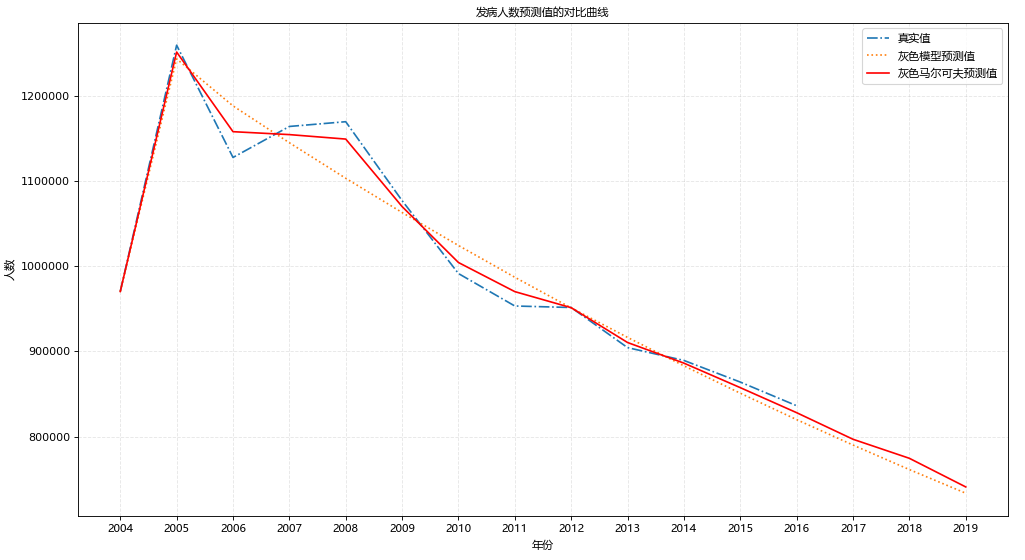
\includegraphics[width=\textwidth]{figures/f.png}
%	\caption{???????????}\label{afd}
%\end{figure}


Similarly, the calculation of the medical demand forecast value for 2009-2018 is obtained as follows:
\begin{gather}
\widehat{X}(k+1)=-???e^{-???k}+???,k=1,2,\cdots,10
\end{gather}



The error status range is shown in the table ~\ref{ss}~.
\begin{table}[htbp]
	\centering\caption{Medical demand status interval division}\label{ss}
	\begin{tabular}{cccc}
		\toprule[1.5pt]
		{\centering Status}
		& {\centering $E_{1}$}
		& {\centering $E_{2}$}
		& {\centering $E_{3}$}
		\\
		\midrule[0.5pt]
		Residual interval &  $[-???,-???]$  &$(-???,???]$ & $(???,???]$   \\ 
		\bottomrule[1.5pt]	
	\end{tabular}
\end{table}

The medical demand forecast is classified into the error interval as shown in the table ~\ref{sss}~:
\begin{table}[htbp]
	\centering\caption{Medical demand error status interval}\label{sss}
	\begin{tabular}{ccccccccccc}
	\toprule[1.5pt]
	{\centering year}
	& {\centering 2009}
	&{\centering 2010}
	& {\centering 2011}
	&{\centering 2012}
	& {\centering 2013}
	& {\centering 2014}
	&{\centering 2015}
	&{\centering 2016}
	&{\centering 2017}
	&{\centering 2018}
	\\
	\midrule[0.5pt]
	Residual interval &  $E_{2}$  &$E_{2}$ & $E_{1}$&$E_{2}$ &$E_{3}$ &$E_{2}$&$E_{1}$&$E_{1}$&$E_{2}$&$E_{2}$\\ 
	\bottomrule[1.5pt]	
\end{tabular}
\end{table}
From this, the initial state probability vector $t_{0}$ is obtained, and the transfer matrix $P$ is:
\begin{gather}
\begin{matrix}
t_{0}'=[???,???,???]\\ 
\\ 
P'=\left(\begin{array}{lll} ??? & ??? & ???\\ ??? & ??? & ??? \\??? & ??? & ???\end{array}\right)
\end{matrix}
\end{gather}

The predicted solution obtained by gray prediction and Markov correction is shown in the figure ~\ref{asf}~.
%\begin{figure}[H]
%	\centering
%	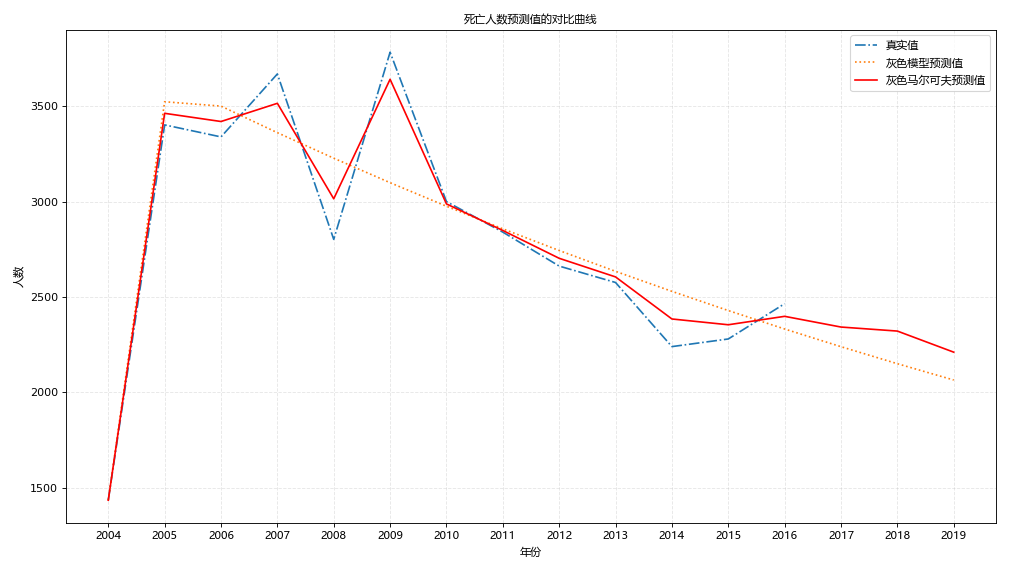
\includegraphics[width=\textwidth]{figures/s.png}
%	\caption{???????????}\label{asf}
%\end{figure}


\subsubsection{Conclusion}
 \subsection{The model of Problem 2}
\subsection{The model of Problem 3}
	\subsubsection{Establishment of model}  
	 \paragraph{ $M/M/c/\infty$ model}
As the theory of$M/M/c/\infty$ illusteate:
\begin{gather}
\left\{\begin{array}{ll}{P_{0}=} & {\left[\sum_{k=0}^{-1} \frac{1}{k !}\left(\frac{\lambda}{\mu}\right)^{k}+\frac{1}{c !} \cdot \frac{1}{1-\rho} \cdot\left(\frac{\lambda}{\mu}\right)^{c}\right]^{-1}} \\ {P_{n}=} & {\left\{\begin{array}{ll}{\frac{1}{n !}\left(\frac{\lambda}{\mu}\right)^{n} P_{0}} & {(n \leqslant c)} \\ {\frac{1}{c ! c^{n-c}}\left(\frac{\lambda}{\mu}\right)^{n} P_{0}} & {(n>c)}\end{array}\right.}\end{array}\right.
\end{gather}
In the above expression, n is the amount of patient.$p_{n}$ is the probability of number of patient reach n in the moment t. C represents the amount of doctors in an outpatient department. $\lambda$ means the average arrival rate of patients. And the $\mu$ means the average inspection rate of the doctor.

Based on this theory, the following relation is set up:       
\begin{gather}
\left\{\begin{array}{l}{L_{s}=L_{q}+\frac{\lambda}{\mu}} \\ {L_{q}=\sum_{n=c+1}^{\infty}(n-c) P_{n}=\frac{\left(c_{\rho}\right)^{c} \rho}{c !(1-\rho)^{2}} P_{0}}\end{array}\right.
\end{gather}
In the above expression, $L_{s}$ is the average length of the queuing which means the number of patient waiting in the system. Depending on it, we could derive the expression of average waiting time $W_{q}$ and average time of stay $W_{s}$:
\begin{gather}
\left\{\begin{matrix}W_{q}=\frac{L_{q}}{\lambda }
\\ W_{s}=\frac{L_{s}}{\lambda }
\end{matrix}\right.
\end{gather}
	\subsubsection{Solution of model}
\paragraph{Optimized systems design} 
For $M/M/c/\infty$ system, the expection of the social cost per hour in the steady state is set up as $Z$. And $Z$ could be calculated as the following expression:     
 \begin{gather}
 z=c_{s} \cdot c+c_{w} \cdot L_{s}
 \end{gather}
 In this expression, $C$ is the number of doctors in the outpatient department. $C_(s)$ represents the average hourly wage of the doctors while $C_(w)$ represents the patient's.$L_{s}$ is the amount of patient waiting in the system witch is function of $C$.Thus ,$Z$ is the function of $C$. To get the optimal solution of $C^*$ which make $Z$ the minimum, we adopt the marginal analysis to solve it.And accroding to the feature that $Z$ is the minimum, the following relation exists:  
\begin{gather}
\left\{\begin{matrix}Z(c^*)\leqslant Z(c^*-1)
\\ Z(c^*)\leqslant Z(c^*+1)
\end{matrix}\right.
\end{gather}
 Take expression (15) into expression (16) to gain:
  \begin{gather}
L(C^*)-L(C^*+1)\leqslant \frac{C_(s)}{C_(w)}\leqslant L(C^*-1)-L(C^*)
 \end{gather}
Thus, we utilize the ergodic algorithm to obtain the value of $C^*$.
\subsection{The model of Problem 4}

%===========================  \section{Sensitivity Analysis}===============================
  \section{Sensitivity Analysis}

%====================================\input{StrengthsandWeaknesses}============================================
\section{Strengths and Weaknesses}

\subsection{Strengths}
\begin{enumerate}
\item Vibration of bat is taken into account so that the accuracy of the model can be fairly good.
\item Physical explanation is put forward besides the model for a better understanding of the collision process.
\item Figures are used for explanation of the problem,thus making it more intuitive and easier to understand.
\end{enumerate}

\subsection{Weaknesses}
\begin{enumerate}
\item The ball is actually nonlinear when deformation of the ball go beyond a certain limit.The approximation of linear model turned to be flawed when the force applied on the ball become very large.
\item Effective coefficient of restitution can not be calculated accurately.This affect the accuracy of the result of the model.
\end{enumerate}

\section{Conclusion}
%========================Bibtex
\newpage
	\nocite{*}		%??????????
%\bibliography{wenxian.bib}
%	%???????wenxian.bib?????
%	
\begin{thebibliography}{9}%??9
	\bibitem{bib:one}Saad Ahmed Javed,Sifeng Liu. Correction to: Predicting the research output/growth of selected countries: application of Even GM (1, 1) and NDGM models[J]. Scientometrics,2019,120(3).
	\bibitem{bib:2}???,???,???.?????????????????[J].??????,2018(15):74-75.	
	\bibitem{bib:3}Yawen Wang,Zhongzhou Shen,Yu Jiang. Analyzing maternal mortality rate in rural China by Grey-Markov model[J]. Medicine,2019,98(6).
	\bibitem{bib:4}Saad Ahmed Javed,Sifeng Liu. Correction to: Predicting the research output/growth of selected countries: application of Even GM (1, 1) and NDGM models[J]. Scientometrics,2019,120(3).
	\bibitem{bib:5}??,???,???.??????GM(1,N)-Markov???????[J].??????,2019(03):43-48.
	\bibitem{bib:6}???,???,???,???.??GM(1,1)?????????GM(1,1)????????????????[J].???????,2011,45(09):1075-1079.
	\bibitem{bib:7}Kate Childs,Christopher Davis,Mary Cannon,Sarah Montague,Ana Filipe,Lily Tong,Peter Simmonds,Donald Smith,Emma C. Thomson,Geoff Dusheiko,Kosh Agarwal. Suboptimal SVR rates in African patients with atypical Genotype 1 subtypes: implications for global elimination of Hepatitis C[J]. Journal of Hepatology,2019.
	\bibitem{bib:8}Yuyan Cao. Failure Prognosis for Electro-Mechanical Actuators Based on Improved SMO-SVR Method[A]. ?????????????????????????????????IEEE??????????.Proceedings of 2016 IEEE Chinese Guidance, Navigation and Control Conference (IEEE CGNCC2016)[C].2016:6.
\end{thebibliography}

\newpage
%??
%\appendix %%??

\end{document}
